\documentclass[10pt,a4paper]{article}
\usepackage[T1]{fontenc}
\usepackage{lmodern}
\usepackage[margin=2.0cm]{geometry}
\usepackage{amsmath}
\usepackage{graphicx}
\usepackage{booktabs}
\usepackage{caption}
\usepackage{cite}
\usepackage{url}
\usepackage[hidelinks]{hyperref}
\graphicspath{{figures/}}
\captionsetup{font=small,labelfont=bf}
\setlength{\parskip}{0.35em}

\title{Sparse FFT on Real High-Definition Automotive Radar:\\ A Measurement Study on RADIal\\[0.3em]\large Extended Technical Report}
\author{Daksh Shah\\
Department of Electrical Engineering, National Institute of Technology Rourkela, India\\
\texttt{daksh06shah2006@gmail.com}\\
Code: \url{https://github.com/PLANETORIAN/Sparse-FFT-Radar}}
\date{November 2026}

\begin{document}
\maketitle

\begin{abstract}
\noindent Sparse Fourier transforms can beat the FFT when a spectrum has few nonzero bins. This report tests whether the Doppler FFT of a real high-definition automotive radar is such a case. I built the range-Doppler chain from the raw ADC files of the RADIal dataset, measured how many Doppler peaks a range row holds in three driving scenes, implemented the exactly-sparse FFT of Hassanieh, Indyk, Katabi and Price, and compared it with a dense FFT on synthetic and real rows. Between 63\% and 89\% of range rows have at most 8 peaks, but rows that contain a labelled vehicle have about 36 to 41, because Doppler-division multiplexing repeats every target 12 times. On real rows the sparse FFT kept fewer Doppler peaks than a dense 256-point FFT or an energy-based row skip at every computation cost. The report gives the method, the numbers, the reasons and the limits of each result. A three-page summary is available as a separate short paper.
\end{abstract}

\tableofcontents
\bigskip

\section{Question and Scope}
A frequency-modulated radar turns each frame into a range-Doppler map with two FFT stages. In the RADIal dataset \cite{rebut2022radial} one frame has 512 range samples, 256 chirps and 16 receive channels. The range stage runs $256 \times 16 = 4096$ FFTs of length 512. The Doppler stage runs $512 \times 16 = 8192$ FFTs of length 256. Counting $(N/2)\log_2 N$ multiplications per FFT, the Doppler stage is about 47\% of the total.

Sparse FFT algorithms \cite{hassanieh2012nearly,hassanieh2012simple} compute the $K$ largest coefficients of a length-$N$ spectrum in time that depends on $K$. If a Doppler row holds only a few targets, such an algorithm could replace the dense Doppler FFT. I asked two questions:
\begin{enumerate}
\item How many Doppler peaks does a range row of a real automotive radar hold?
\item Does a sparse FFT, implemented and run on those rows, need less computation than the dense FFT for the same result?
\end{enumerate}

The scope is three sequences of one dataset, one radar, and the Doppler transform size $N = 256$. I did not synthesise hardware. Cost is an operation count.

\section{Dataset and Raw Data Handling}
\subsection{Sequences}
RADIal contains raw ADC data of a high-definition radar with camera, laser scanner, GPS and vehicle labels \cite{rebut2022radial}. I used three sequences (Table~\ref{tab:seq}). The label file has no scene-type column. I chose the sequences from the label statistics and confirmed the scene type from the camera. My first highway choice turned out to be a two-lane rural road, so I replaced it. The final highway sequence has a GPS speed of 107 to 117\,km/h.

\begin{table}[h]
\caption{Sequences used. A complete frame has all four radar chip blocks.}
\label{tab:seq}
\centering
\begin{tabular}{llc}
\toprule
Scene & Sequence & Complete radar frames \\
\midrule
City & \texttt{RECORD@2020-11-21\_13.46.26} & 576 \\
Countryside & \texttt{RECORD@2020-11-22\_12.54.38} & 452 \\
Highway & \texttt{RECORD@2020-11-22\_12.38.47} & 388 \\
\bottomrule
\end{tabular}
\end{table}

\subsection{From log file to data cube}
Each sequence stores the ADC samples of the four radar chips in four binary files. An event log lists, for every block, the sensor, a sample number, the byte offset and the size. I read every block at the offset given by the log. The binary files contain a few more blocks than the log lists, so counting blocks in the file would give wrong frames.

One block is 2\,097\,152 bytes: 1\,048\,576 16-bit values, which are the in-phase and quadrature parts of 512 samples $\times$ 256 chirps $\times$ 4 receive channels. The file order is sample, then channel, then chirp.

A radar frame combines one block of each chip. Following the dataset's reader, a frame anchored at sample number $n$ of chip 3 takes chip 0 at $n+1$, chip 2 at $n+2$ and chip 1 at $n+3$. I stack the channels in the order chip 3, 0, 1, 2 to get a $512 \times 256 \times 16$ complex cube. Grouping the blocks by a fixed count of four did not work, because a recording can start in the middle of a cycle.

\subsection{Dropped blocks}
Some blocks are missing in every sequence. In the countryside sequence, 10 of 462 anchor blocks have no complete set of four chips. I use only complete frames. The gaps matter for the labels: after the first gap, the $k$-th labelled frame and the $k$-th complete frame are no longer the same frame. Section~\ref{sec:vehicle} explains how I avoided this problem.

\section{Baseline Processing Chain}
\subsection{Range-Doppler map}
The chain follows the order of the dataset's signal-processing code, written again from the raw data:
\begin{enumerate}
\item subtract the mean of each channel over samples and chirps;
\item Hamming window and FFT along the 512 samples (range);
\item Hamming window and FFT along the 256 chirps (Doppler).
\end{enumerate}
One range bin is $103/512 \approx 0.2$\,m. For the sparsity study I use the power map
\begin{equation}
P[r, d] = \sum_{c=1}^{16} \left| X_c[r, d] \right|^2 ,
\label{eq:power}
\end{equation}
where $X_c[r,d]$ is the range-Doppler value of channel $c$ at range bin $r$ and Doppler bin $d$. $P$ has $512 \times 256$ bins.

\subsection{Doppler-division multiplexing}
The radar has 12 transmitters that send at the same time. Each one adds its own phase step from chirp to chirp, which shifts its returns along Doppler. A single target therefore appears 12 times in a Doppler row, 16 bins apart, and 4 of the 16 slots stay empty (Fig.~\ref{fig:comb}). I verified the spacing on real rows: local maxima at bins 70, 86, \ldots, 246, every gap exactly 16.

\begin{figure}[h]
\centering
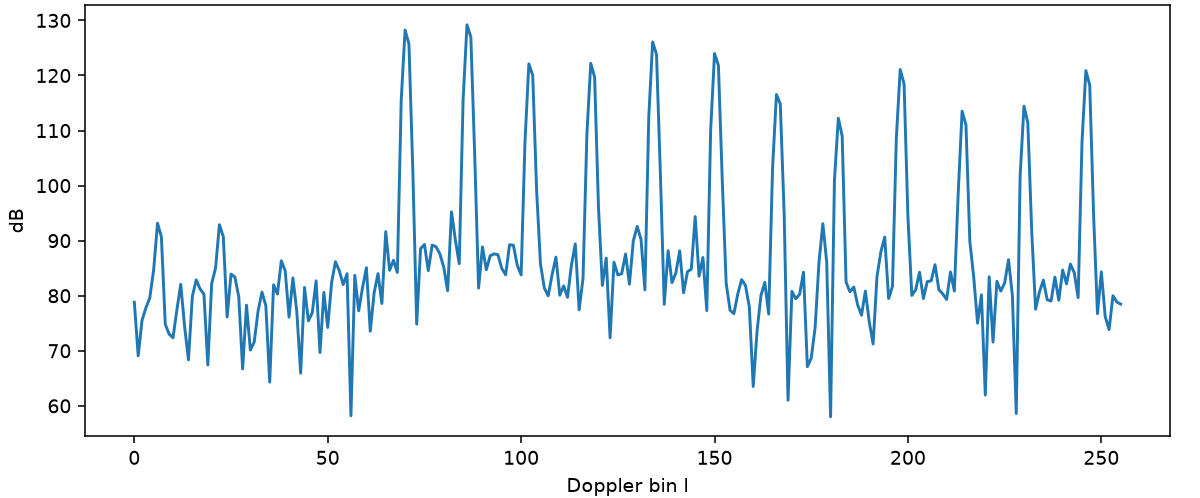
\includegraphics[width=0.8\textwidth]{fig_ddm_comb.png}
\caption{Doppler spectrum (dB against Doppler bin) of one range row with a vehicle, one receive channel. The vehicle appears as 12 copies, 16 bins apart. The band at low bin numbers holds the 4 empty slots.}
\label{fig:comb}
\end{figure}

For detection, the copies can be added by folding the 256 Doppler bins into 16 (bin $d$ goes to $d \bmod 16$). The folded map is $512 \times 16$. I use it only for the detection check below. It is the wrong place to measure sparsity for a Doppler sparse FFT, because the fold is itself computed from the full 256-bin spectrum.

\subsection{CA-CFAR and the check against labels}
I apply cell-averaging CFAR \cite{rohling1983cfar} to the folded map, with 9 training and 3 guard cells on each side in both directions. A cell is detected if its power exceeds the mean of its training cells by a threshold in dB.

To choose the threshold I matched detections to the labelled vehicle ranges of the countryside sequence. A label counts as found if a detection lies within 5 range bins. Because hundreds of detections cover much of the range axis, I also measured a chance level: the share of range bins far from any label that still lie within 5 bins of a detection. Table~\ref{tab:thr} gives both. I fixed the threshold at 4\,dB.

\begin{table}[h]
\caption{CA-CFAR threshold on the countryside sequence (556 labels). Lift = (hit $-$ chance)/(1 $-$ chance).}
\label{tab:thr}
\centering
\begin{tabular}{cccc}
\toprule
Threshold (dB) & Hit rate & Chance level & Lift \\
\midrule
2 & 0.978 & 0.890 & 0.804 \\
4 & 0.951 & 0.710 & 0.832 \\
6 & 0.896 & 0.540 & 0.773 \\
8 & 0.865 & 0.391 & 0.779 \\
10 & 0.815 & 0.285 & 0.741 \\
\bottomrule
\end{tabular}
\end{table}

Two cautions apply to Table~\ref{tab:thr}. The threshold was chosen on the same labels it is measured on. And the table uses a simple label-to-frame mapping that is wrong for some frames after a dropped block, so the hit rates are probably slightly low. The table supports the choice of 4\,dB. It is not a detector benchmark. No result in the following sections depends on it.

\subsection{Camera pairing}
The camera stream is a sequence of JPEG images listed in the same event log. I paired each radar frame with the image whose time of issue is closest. With this pairing the dataset's label boxes lie on the vehicles (Fig.~\ref{fig:camera}). With the fixed sensor delay that the dataset's reader offers as another mode, the boxes lay beside the vehicle on the frames I checked. I do not know why, and I describe the pairing only as the one under which the labels fit.

\begin{figure}[h]
\centering
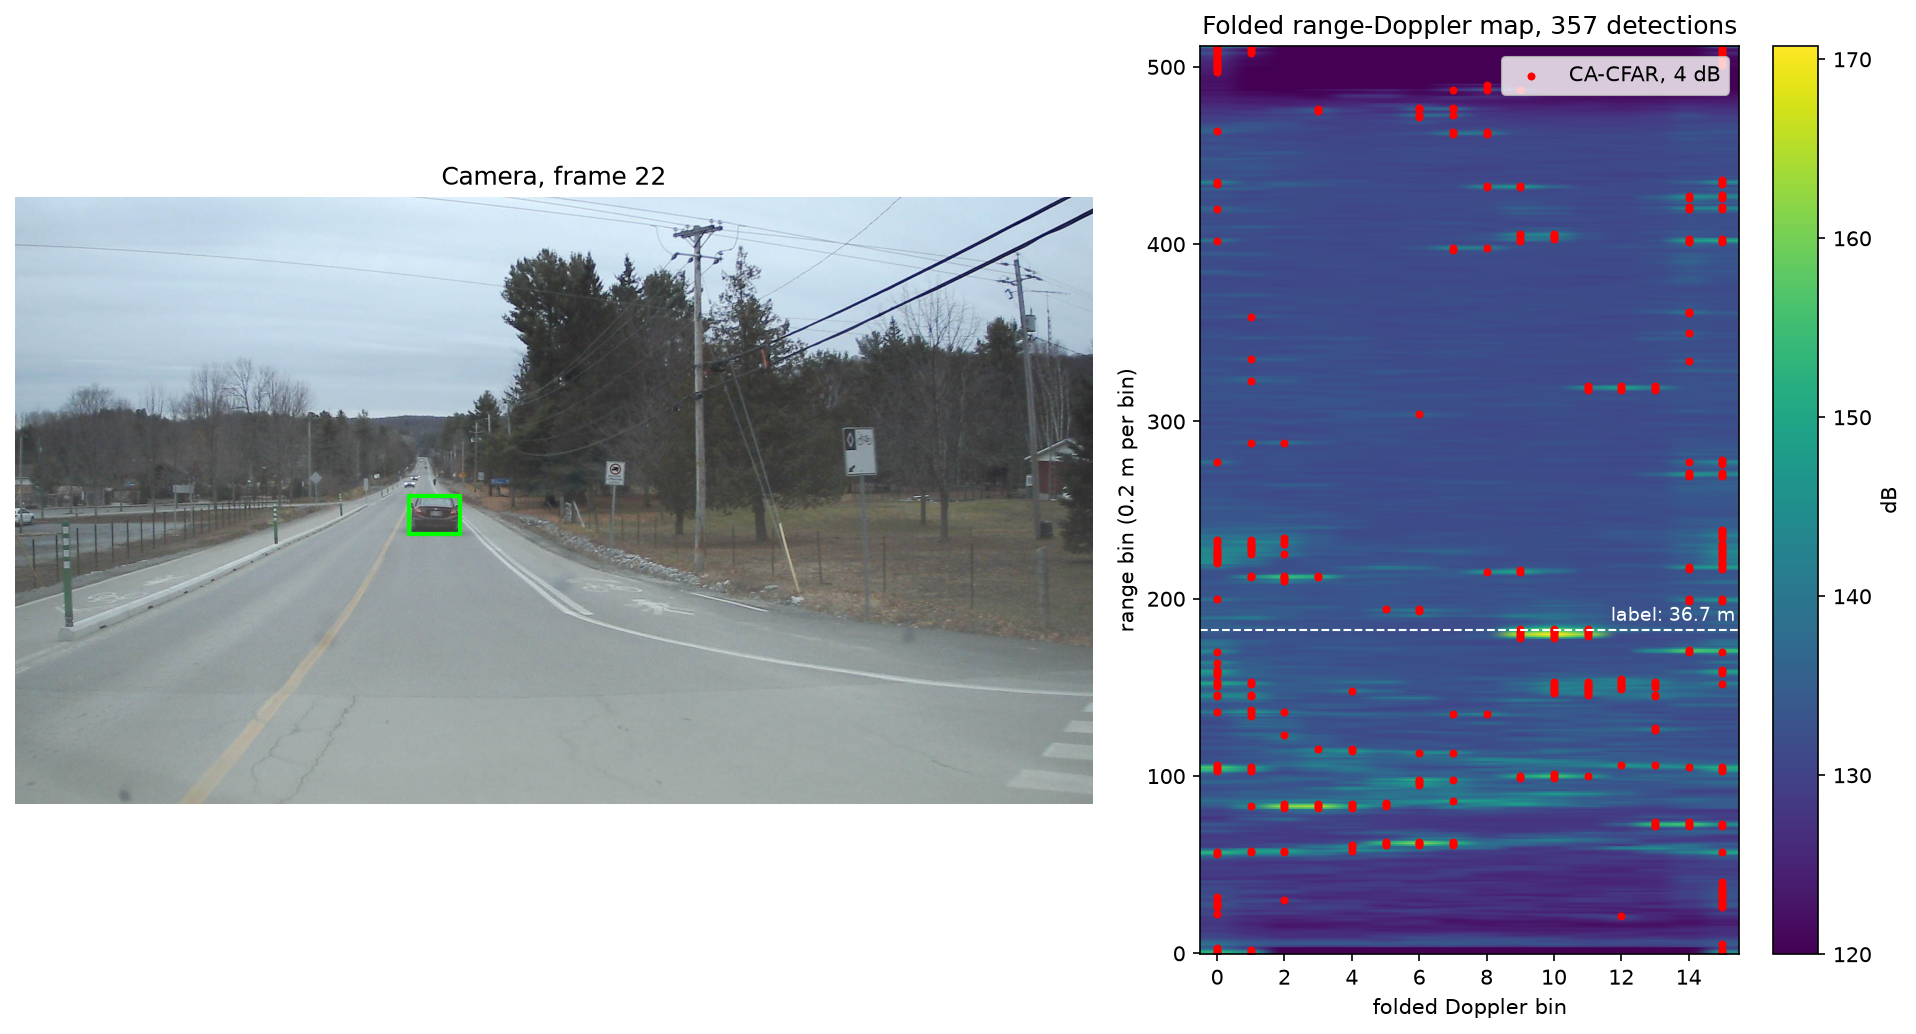
\includegraphics[width=0.9\textwidth]{fig_camera_rd_cfar.png}
\caption{Check of the chain on one countryside frame. Left: camera image with the dataset's label box. Right: folded range-Doppler map with CA-CFAR detections at 4\,dB (red) and the labelled range of 36.7\,m (dashed). The brightest return lies at the labelled range. Detections in the edge columns are mostly static clutter, which is not removed.}
\label{fig:camera}
\end{figure}

I repeated this check on the first labelled frames of the city and highway sequences. Static clutter was not removed in any experiment. With a moving radar and DDM, the static scene is not at zero Doppler, and subtracting the mean over chirps changed the maps very little.

\section{How Sparse Is Real Radar?}
\subsection{First measure: $K_{90}$, and why it misleads}
My first measure was $K_{90}$, the smallest number of bins of $P$ that hold 90\% of its total energy. As a control I passed complex Gaussian noise through the same windows, FFTs and channel sum.

\begin{table}[h]
\caption{Whole-map measures on the first frame of each sequence. Shares are of the 131\,072 bins.}
\label{tab:k90}
\centering
\begin{tabular}{lccccc}
\toprule
 & $K_{50}$ & $K_{90}$ & $K_{99}$ & Floor share & Bins $>10$\,dB above median \\
\midrule
City & 0.12\% & 5.3\% & 59.8\% & 0.055 & 11\,723 (8.9\%) \\
Countryside & 0.06\% & 13.3\% & 75.1\% & 0.128 & 4369 (3.3\%) \\
Highway & 0.34\% & 46.1\% & 84.8\% & 0.291 & 3238 (2.5\%) \\
Noise control & -- & 84.6\% & -- & -- & 0 \\
\bottomrule
\end{tabular}
\end{table}

$K_{90}$ ranks the scenes backwards (Table~\ref{tab:k90}). It calls the city the sparsest scene and the highway the least sparse, although the highway frame shows one vehicle on an open road. The reason is the noise floor. I estimated its share of the total energy as the median bin power times the number of bins, divided by the total. On the highway the floor holds about 29\% of the energy, so the peaks hold only about 71\%. To reach 90\%, $K_{90}$ has to collect tens of thousands of nearly equal floor bins. $K_{90}$ measures how energy splits between peaks and floor. It does not count peaks. Counting the bins more than 10\,dB above the median gives the expected order.

The noise control also corrected a wrong expectation of mine. A single channel of complex noise needs about 59\% of its bins for 90\% of its energy. I expected the same for the map. But $P$ sums 16 channels, which makes the noise bins nearly equal, and the control gave 84.6\%.

\subsection{Peaks per range row}
A Doppler sparse FFT would replace one 256-point FFT per range row. I therefore define, for each range row,
\begin{equation}
K[r] = \#\left\{ d : P[r,d] > 10 \cdot \operatorname{median}_d P[r,d] \right\},
\label{eq:k}
\end{equation}
the number of Doppler bins more than 10\,dB above the median of that row. Using the median of each row accounts for a noise floor that changes with range. The noise control gives $K = 0$ in every row.

\begin{figure}[h]
\centering
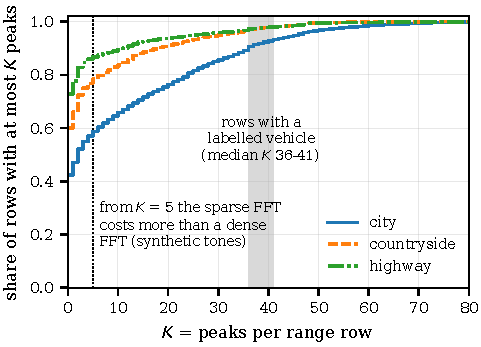
\includegraphics[width=0.62\textwidth]{fig_row_k_cdf.pdf}
\caption{Share of range rows with at most $K$ Doppler peaks, Eq.~\eqref{eq:k}, pooled over every 5th frame of each sequence. Most rows are nearly empty. Rows with a labelled vehicle lie in the grey band.}
\label{fig:cdf}
\end{figure}

\begin{table}[h]
\caption{Peaks per range row, every 5th frame, all 512 rows per frame.}
\label{tab:rowk}
\centering
\begin{tabular}{lccc}
\toprule
 & City & Countryside & Highway \\
\midrule
Frames / rows & 116 / 59\,392 & 91 / 46\,592 & 78 / 39\,936 \\
\multicolumn{4}{l}{\emph{Threshold 10\,dB}} \\
Median $K$ & 2 & 0 & 0 \\
90th percentile & 36 & 18 & 11 \\
Maximum & 108 & 85 & 96 \\
Rows with $K = 0$ & 42\% & 60\% & 73\% \\
Rows with $K \le 8$ & 63.2\% & 81.9\% & 88.5\% \\
\multicolumn{4}{l}{\emph{Threshold 6\,dB}} \\
Median $K$ & 16 & 6 & 1 \\
90th percentile & 54 & 39 & 29 \\
Rows with $K = 0$ & 22.3\% & 31.2\% & 46.3\% \\
Rows with $K \le 8$ & 39.9\% & 56.6\% & 71.4\% \\
\bottomrule
\end{tabular}
\end{table}

Fig.~\ref{fig:cdf} and Table~\ref{tab:rowk} give the result. The distribution is very skewed. Most rows are empty or nearly empty, and a minority are crowded, with up to 108 of 256 bins above the threshold. The first frame of each sequence was busier than the average, so one frame would have been misleading. The order of the scenes is the same at 10\,dB and 6\,dB. The absolute shares are not: they move by about 20 points. Any statement of $K$ needs its threshold.

\subsection{Rows that contain a vehicle}
\label{sec:vehicle}
Fig.~\ref{fig:cdf} mixes rows with and without targets. To separate them I looked up $K$ in the rows where the dataset labels a vehicle. I used only labelled frames before the first dropped radar block of a sequence, where the label index and the frame index agree.

A first attempt looked at the label's range bin and its two neighbours. It gave $K \approx 36$ in the countryside but $K = 0$ on the highway. Printing $K$ for the rows around each highway label showed the reason: the vehicle's rows lie 6 to 11 bins beyond the labelled range. I then searched the busiest row within 20 bins of each label and recorded its offset from the label.

\begin{table}[h]
\caption{$K$ in rows with a labelled vehicle (10\,dB). Vehicles within 5 bins of their scene's median offset.}
\label{tab:vehicle}
\centering
\begin{tabular}{lccc}
\toprule
 & City & Countryside & Highway \\
\midrule
Vehicles used & 1 & 55 & 32 \\
Median $K$ & (too few) & 41 & 36 \\
Maximum $K$ & -- & 69 & 48 \\
Vehicle rows with $K \le 8$ & -- & 0\% & 0\% \\
Median offset from label (bins) & -- & 0 & $+9$ \\
\bottomrule
\end{tabular}
\end{table}

A row with a vehicle holds about 36 to 41 peaks (Table~\ref{tab:vehicle}), and none of the 87 vehicle rows had 8 or fewer. The number is what DDM predicts: 12 copies, each about 3 bins wide after the Hamming window. So the sparse rows of Fig.~\ref{fig:cdf} are the rows without targets. A sparse FFT that only wins on those rows competes with a much simpler idea: do not transform empty rows at all.

\subsection{An offset between labels and radar on the highway}
On the highway the radar sees the labelled vehicle about 9 range bins (about 1.8\,m) beyond the labelled range. In the countryside the offset is 0. A wrong range-bin size would grow with range and would give about 6 bins at the countryside ranges of 40 to 44\,m, which is not observed. A fixed shift would also appear in the countryside. The labels come from the camera and laser scanner, not from the radar frame. My best explanation is a small time difference between the labelled instant and the radar frame I pair with it, which matters only when the vehicle's range changes from frame to frame, as it does on the highway. I have not tested this explanation. It does not affect the sparsity results, because I locate the vehicle's rows directly. It would affect detection hit rates.

\section{The Sparse FFT, Step by Step}
I implemented the algorithm for exactly sparse signals from the paper of Hassanieh, Indyk, Katabi and Price \cite{hassanieh2012nearly}. It is the simplest of their algorithms. Real radar rows are not exactly sparse, and seeing where that assumption breaks was part of the aim. The code is in \texttt{src/sfftradar/sfft.py}. Throughout, $N = 256$ is the row length and $B$ the number of buckets, with $L = N/B$ bins per bucket.

\subsection{Why simple buckets fail on this radar}
The textbook way to form $B$ buckets is to keep every $L$-th sample and take a $B$-point FFT. Bin $f$ then lands in bucket $f \bmod B$. With $B = 16$ this adds exactly the bins that are 16 apart, so all 12 DDM copies of a target fall into one bucket. The location step below needs at most one tone per bucket, so this bucketing cannot work on a DDM radar. The algorithm of \cite{hassanieh2012nearly} uses buckets that are bands of neighbouring bins, after a random permutation. Both parts are needed.

\subsection{Permutation}
Reading the samples as $y[m] = x[\sigma m \bmod N]$ with an odd $\sigma$ moves every tone from bin $f$ to bin $\sigma f \bmod N$. No FFT is involved, only a different reading order. The permutation is undone for a found bin $p$ by $f = \sigma^{-1} p \bmod N$. $\sigma$ must be odd so that the inverse exists for $N = 256$. A new random $\sigma$ in each round means that two tones that share a bucket once will probably not share it again.

\subsection{Flat window}
\label{sec:window}
To make a bucket a band of neighbouring bins, the samples are multiplied by a window $w$ whose spectrum $G$ is close to 1 over $L$ neighbouring bins and close to 0 elsewhere. I design $G$ as a box of width $L$ with edges rounded by an error function, transform it to time, and set time samples below 0.1\% of the peak to zero (Fig.~\ref{fig:window}). The rounding of the edges trades flatness against window length (Table~\ref{tab:window}). I used an edge parameter of 1.5.

\begin{figure}[h]
\centering
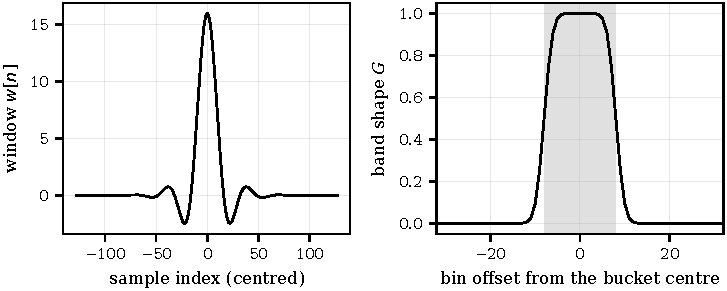
\includegraphics[width=0.85\textwidth]{fig_flat_window.pdf}
\caption{Flat window for $N = 256$, $B = 16$. Left: the time window, of which 141 samples are nonzero. Right: its spectrum, the shape of one bucket. The grey band is the 16 bins the bucket should cover.}
\label{fig:window}
\end{figure}

\begin{table}[h]
\caption{Flat window, $N = 256$, $B = 16$: edge rounding against length.}
\label{tab:window}
\centering
\begin{tabular}{ccc}
\toprule
Edge parameter (bins) & Nonzero samples & Lowest value of $G$ within 5 bins of the centre \\
\midrule
1.0 & 199 & 0.998 \\
1.5 & 141 & 0.977 \\
2.0 & 113 & 0.933 \\
\bottomrule
\end{tabular}
\end{table}

This table already shows the main cost problem at this size. A single hashing reads 141 of the 256 samples. For $B = 32$ and $B = 64$ the window has 161 and 175 nonzero samples.

\subsection{Hashing into buckets}
One hashing with permutation $\sigma$ and shift $\tau$ computes
\begin{equation}
u_\tau[j] = \sum_{i=0}^{B-1} \Bigl( \sum_{k=0}^{L-1} w[i + kB]\; x[\sigma(i + kB + \tau) \bmod N] \Bigr) e^{-2\pi \mathrm{i}\, i j / B}, \qquad j = 0, \ldots, B-1 .
\label{eq:hash}
\end{equation}
The inner sum multiplies by the window and folds the $N$ products into $B$ values. The outer sum is one $B$-point FFT. The result is that bucket $j$ holds the permuted bins near $jL$, each weighted by $G$:
\begin{equation}
u_0[j] = \sum_{p} Y[p]\; G[p - jL],
\end{equation}
where $Y$ is the spectrum of the permuted row. I checked the implementation against this formula with a full FFT; they agree to $6 \times 10^{-14}$. I also checked that the 12 DDM copies of one target land in 12 different buckets.

\subsection{Locating a tone}
If bucket $j$ holds a single tone at permuted bin $p$, a shift by one sample multiplies its value by $e^{2\pi \mathrm{i} p / N}$, and the window weight cancels in the ratio. So
\begin{equation}
\hat{p} = \operatorname{round}\!\left( \frac{N}{2\pi} \arg \frac{u_1[j]}{u_0[j]} \right), \qquad \hat{f} = \sigma^{-1} \hat{p} \bmod N, \qquad \hat{X}[\hat{f}] = \frac{u_0[j]}{G[\hat{p} - jL]} .
\label{eq:locate}
\end{equation}
Two tests reject buckets that hold more than one tone: the ratio must have a magnitude close to 1, and $\hat{p}$ must lie inside the band of bucket $j$. The second test also rejects the leakage of a tone into a neighbouring bucket. Neither test is perfect. In a test row with tones at bins 27, 66, 76, 105 and 211, two tones shared a bucket, passed both tests and produced a false tone at bin 229.

\subsection{Rounds}
The full algorithm repeats: choose a random odd $\sigma$, locate the tones that are alone in a bucket, subtract them from the row, and continue on the remainder. Estimates for the same bin are added over rounds, so a false tone is cancelled when a later round finds its negative. On the test row above, all five tones were recovered exactly after a few rounds, and the false tone disappeared.

\subsection{Changes needed for real rows}
Two changes were necessary before the algorithm produced anything useful on RADIal rows.

\emph{All channels together.} The map $P$ of Eq.~\eqref{eq:power} sums 16 channels. A target that is clear in $P$ can be weak in a single channel. I hash all channels with the same $\sigma$, sum the bucket power over channels to decide which buckets are occupied, and average the phase over channels as $\arg \sum_c u_{1,c}[j]\, u_{0,c}^*[j]$. A tone turns by the same angle in every channel.

\emph{A threshold relative to noise.} A real row is never exactly sparse. Every bucket holds noise, and with the threshold used for synthetic rows the algorithm reported a tone in almost every bin. I call a bucket occupied if its power exceeds $c$ times the median bucket power, and I stop when a round finds nothing. The parameter $c$ is studied in Section~\ref{sec:checks}.

\section{Synthetic Rows and the Cost Model}
\subsection{Cost model}
I count complex multiplications. A dense radix-2 FFT of length $N$ costs $(N/2)\log_2 N$, which is 1024 for $N = 256$. One hashing costs the number of nonzero window samples plus $(B/2)\log_2 B$. One round is two hashings plus two multiplications per bucket. This gives 378, 546 and 862 multiplications per round for $B = 16$, 32 and 64. The subtraction of found tones is counted as free. The paper subtracts inside the buckets; my implementation subtracts in time, which would cost more. The model therefore favours the sparse FFT.

\subsection{Result}
I generated rows with $K$ tones on exact bins, with random complex amplitudes and no noise, and counted a trial as a success if every bin was recovered to within 1\% of the largest coefficient.

\begin{table}[h]
\caption{Synthetic rows, 100 trials per entry: share recovered / median multiplications. Dense FFT: 1024.}
\label{tab:syn}
\centering
\begin{tabular}{lcccccc}
\toprule
$B$ & $K = 1$ & $K = 5$ & $K = 8$ & $K = 12$ & $K = 20$ & $K = 36$ \\
\midrule
16 & 1.00 / 378 & 1.00 / 1512 & 1.00 / 2646 & 0.93 / 4536 & 0.09 / 4536 & 0.00 / 4536 \\
32 & 1.00 / 546 & 1.00 / 1638 & 1.00 / 2730 & 1.00 / 6552 & 0.98 / 6552 & 0.00 / 6552 \\
64 & 1.00 / 862 & 1.00 / 2586 & 1.00 / 3448 & 1.00 / 10\,344 & 1.00 / 10\,344 & 0.91 / 10\,344 \\
\bottomrule
\end{tabular}
\end{table}

Table~\ref{tab:syn} shows that the sparse FFT is cheaper than the dense FFT for one tone and already more expensive for five. I did not measure $K = 2$ to 4, so the break-even lies somewhere in that range. Before this experiment I had guessed a break-even near $K = 8$; that was too optimistic. A row with 36 tones, the vehicle-row case, needs $B = 64$, costs about ten times the dense FFT, and still fails in 9\% of trials. These are the most favourable conditions: tones on exact bins and no noise.

\section{Real Rows}
\subsection{Method}
For each frame I compute the range FFT and the Doppler window as in the baseline, which gives, for each range row, 256 samples in 16 channels. The reference is the dense Doppler FFT of that row and its power $P[r, \cdot]$. A dense peak is a local maximum of $P[r, \cdot]$ more than 10\,dB above the row median. The sparse FFT returns a set of bins with a value per channel; I sum their power over channels. A dense peak counts as kept if the sparse output exceeds the same threshold at the peak's bin or a neighbouring bin. Cost is the multiplications per row from the model above, divided by 1024. I used every 25th frame of each sequence and all 512 rows.

\subsection{Result}
\begin{table}[h]
\caption{Real rows, $c = 4$: share of dense peaks kept / cost relative to a dense FFT.}
\label{tab:real}
\centering
\begin{tabular}{lccc}
\toprule
 & $B = 16$ & $B = 32$ & $B = 64$ \\
\midrule
City & 0.03 / 0.51 & 0.24 / 1.29 & 0.61 / 2.99 \\
Countryside & 0.04 / 0.46 & 0.27 / 0.98 & 0.60 / 2.12 \\
Highway & 0.07 / 0.46 & 0.35 / 0.85 & 0.70 / 1.70 \\
\bottomrule
\end{tabular}
\end{table}

With 16 buckets the sparse FFT costs half a dense FFT and keeps almost nothing (Table~\ref{tab:real}). With 64 buckets it keeps 60\% to 70\% of the peaks at 1.7 to 3 times the dense cost.

\subsection{Why the recall is low}
Two effects explain Table~\ref{tab:real}. The first is the number of peaks in a row with a target, about 36, which Table~\ref{tab:syn} shows to be beyond what 16 or 32 buckets can separate.

The second effect does not appear in noise-free tests. A bucket sums $L$ neighbouring bins, so it also sums $L$ bins of noise. A peak that stands 10\,dB above the noise of its own bin is compared, inside the bucket, with
\begin{equation}
10 \log_{10} L \ \text{dB}
\end{equation}
more noise: 12\,dB for $B = 16$, 9\,dB for $B = 32$ and 6\,dB for $B = 64$. A 10\,dB peak is below the noise of a 16-bin bucket and cannot be found. This matches the steady rise of recall with $B$.

\section{Two Checks}
\label{sec:checks}
\subsection{Does the threshold $c$ change the conclusion?}
\begin{table}[h]
\caption{Effect of the occupancy threshold $c$ (every 25th frame, every 4th row): peaks kept / relative cost.}
\label{tab:c}
\centering
\begin{tabular}{llccc}
\toprule
$c$ & Scene & $B = 16$ & $B = 32$ & $B = 64$ \\
\midrule
2 & City & 0.30 / 2.04 & 0.70 / 4.16 & 0.92 / 8.12 \\
 & Countryside & 0.31 / 1.83 & 0.70 / 3.87 & 0.93 / 7.77 \\
 & Highway & 0.36 / 1.45 & 0.74 / 3.23 & 0.95 / 6.74 \\
\midrule
4 & City & 0.03 / 0.50 & 0.24 / 1.26 & 0.62 / 3.00 \\
 & Countryside & 0.04 / 0.46 & 0.28 / 1.04 & 0.59 / 2.14 \\
 & Highway & 0.06 / 0.44 & 0.35 / 0.87 & 0.67 / 1.69 \\
\midrule
8 & City & 0.00 / 0.38 & 0.06 / 0.67 & 0.28 / 1.60 \\
 & Countryside & 0.01 / 0.38 & 0.09 / 0.62 & 0.27 / 1.19 \\
 & Highway & 0.01 / 0.38 & 0.14 / 0.62 & 0.34 / 1.12 \\
\bottomrule
\end{tabular}
\end{table}

A lower threshold finds more peaks and needs more rounds (Table~\ref{tab:c}). With $c = 2$ and 64 buckets the sparse FFT keeps 92\% to 95\% of the peaks, at 6.7 to 8.1 times the dense cost. With $c = 8$ it is cheap and keeps little. The threshold moves the algorithm along one trade-off curve. No setting keeps most peaks for less than the dense cost.

\subsection{A realistic row skip}
The comparison I had in mind after Section~\ref{sec:vehicle} was a perfect skip of empty rows, which would keep every peak and cost as much as the share of rows with a peak: 0.57, 0.40 and 0.28 of the dense cost in the three scenes. A real system does not know in advance which rows are empty. I therefore tested a skip that it could build: compute the energy of each row, $\sum |x|^2$ over chirps and channels, and run the dense FFT only where the energy exceeds $a$ times the median row energy. I charge 0.125 of a dense FFT per row for the energy test.

\begin{table}[h]
\caption{Energy-based row skip: peaks kept / relative cost.}
\label{tab:skip}
\centering
\begin{tabular}{lccccc}
\toprule
 & $a = 1.0$ & $a = 1.2$ & $a = 1.5$ & $a = 2.0$ & $a = 3.0$ \\
\midrule
City & 0.82 / 0.62 & 0.79 / 0.54 & 0.74 / 0.47 & 0.67 / 0.41 & 0.56 / 0.34 \\
Countryside & 0.79 / 0.62 & 0.78 / 0.50 & 0.74 / 0.42 & 0.65 / 0.35 & 0.52 / 0.27 \\
Highway & 0.70 / 0.62 & 0.69 / 0.46 & 0.65 / 0.35 & 0.55 / 0.27 & 0.43 / 0.21 \\
\bottomrule
\end{tabular}
\end{table}

The perfect skip was too optimistic. Even with $a = 1$, which transforms half of the rows, the energy test loses 18\% to 30\% of the peaks (Table~\ref{tab:skip}). Weak peaks sit in rows whose total energy is below the median. Still, at about 0.6 of the dense cost the energy skip keeps 70\% to 82\% of the peaks, where the sparse FFT keeps 6\% to 14\%.

\begin{figure}[h]
\centering
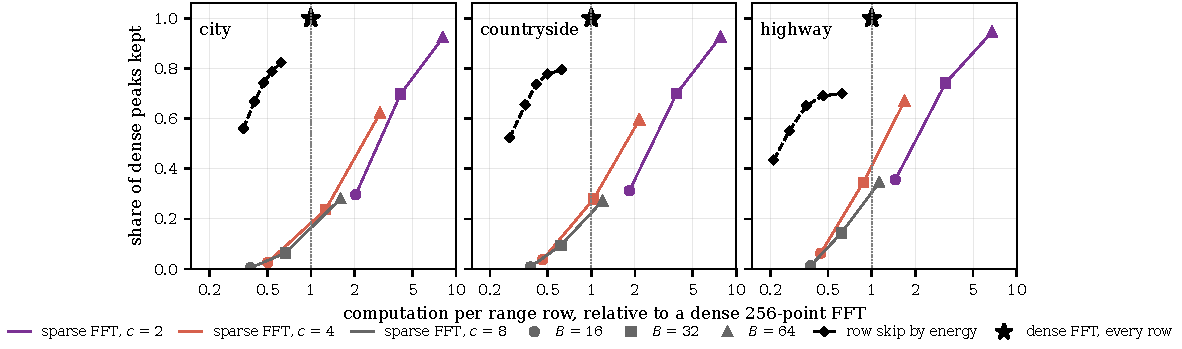
\includegraphics[width=\textwidth]{fig_recall_vs_cost.pdf}
\caption{All real-row results. Share of dense Doppler peaks kept against computation per range row relative to a dense 256-point FFT. Colour: threshold $c$; marker: number of buckets $B$; dashed: energy-based row skip for $a = 3$ to 1; star: dense FFT on every row. In every scene the sparse FFT lies below and to the right of both alternatives.}
\label{fig:recall}
\end{figure}

Fig.~\ref{fig:recall} collects the results. In all three scenes the sparse FFT is dominated: for any of its points there is a cheaper alternative that keeps more peaks. The figure also shows a second finding. The simple shortcut loses peaks too, so at this size the dense FFT on every row is hard to improve on.

\section{Conclusions, Limitations and Next Steps}
\subsection{What the measurements show}
\begin{enumerate}
\item Most range rows of a real HD radar are sparse in Doppler: 63\% to 89\% have at most 8 peaks at 10\,dB.
\item The rows that matter are not. A row with a vehicle holds about 36 to 41 peaks, because DDM repeats each target 12 times.
\item An exactly-sparse FFT at $N = 256$ is cheaper than a dense FFT only for very few tones, even on ideal synthetic rows, because its window reads more than half of the samples per hashing.
\item On real rows it keeps fewer peaks than a dense FFT or an energy-based row skip at every cost. Besides the number of peaks, each bucket collects the noise of all its bins, which hides weak peaks.
\end{enumerate}

\subsection{Limitations}
\begin{itemize}
\item Three sequences of one dataset and one radar. Sparsity used every 5th frame; the sparse FFT comparison used every 25th frame.
\item $K$ depends on its threshold. I report 10\,dB and 6\,dB; the ranking of scenes is stable, the absolute shares are not.
\item The vehicle-row result rests on 55 and 32 vehicles from the early part of two sequences. The city sequence left one usable vehicle.
\item The reference is the set of dense peaks above 10\,dB, not a list of true targets. Static clutter is included.
\item I tested the exactly-sparse algorithm. The noise-tolerant algorithms of \cite{hassanieh2012nearly,hassanieh2012simple} may keep more peaks, at a higher cost.
\item Tones were located with a single shift. I did not test off-grid tones or noise on synthetic rows separately.
\item The cost is a count of complex multiplications. Memory access, control logic, word lengths and latency are not included, and no design was synthesised.
\item The offset between highway labels and radar returns is unexplained.
\end{itemize}

\subsection{Next steps}
\begin{itemize}
\item \emph{A DDM-aware sparse transform.} The 12 copies of a target have a known spacing. An algorithm that treats them as one target would face one group per vehicle instead of about 36 separate peaks.
\item \emph{A two-dimensional transform.} Over range and Doppler together the transform size is $512 \times 256$, where the window is a small part of the data and sparse methods have more room.
\item \emph{Hardware measurement.} An HLS implementation of the dense FFT, the energy skip and one sparse stage would replace the operation count with area and latency.
\item \emph{Label timing.} Matching labels to radar frames by time stamps would explain or remove the highway offset and allow a proper detection benchmark.
\end{itemize}

\appendix
\section{Parameters}
\begin{table}[h]
\centering
\begin{tabular}{ll}
\toprule
Quantity & Value \\
\midrule
Cube per frame & 512 samples $\times$ 256 chirps $\times$ 16 receive channels \\
Transmitters & 12, separated by DDM, copies 16 Doppler bins apart \\
Range bin & $103/512 \approx 0.2$\,m \\
Windows & Hamming, range and Doppler \\
CA-CFAR (folded map) & 9 training and 3 guard cells per side, threshold 4\,dB \\
Peak threshold for $K$ & 10\,dB above the row median (6\,dB as a check) \\
Sparse FFT & $N = 256$; $B = 16$, 32, 64; shifts 0 and 1; at most 12 rounds \\
Flat window & edge 1.5 bins, truncation at 0.1\% of the peak; 141 / 161 / 175 samples \\
Occupancy threshold $c$ & 4 (2 and 8 as a check) \\
Collision test & ratio magnitude within 0.2 of 1 (0.1 for synthetic rows) \\
\bottomrule
\end{tabular}
\end{table}

\section{Repository Map}
\begin{table}[h]
\centering
\begin{tabular}{ll}
\toprule
Path & Content \\
\midrule
\texttt{src/sfftradar/radial.py} & event log parser, block reader, frame cube, labels \\
\texttt{src/sfftradar/rd.py} & windows, range-Doppler map, folded map, CA-CFAR, row inputs \\
\texttt{src/sfftradar/sparsity.py} & $K_{90}$, per-row $K$, noise control, peak finder \\
\texttt{src/sfftradar/sfft.py} & flat window, hashing, location, sparse FFT, cost model \\
\texttt{src/sfftradar/evaluate.py} & peaks kept by the sparse FFT on one row \\
\texttt{notebooks/01\_loader.ipynb} & chain from raw data, CFAR, labels, camera (Fig.~\ref{fig:comb}, \ref{fig:camera}) \\
\texttt{notebooks/02\_sparsity.ipynb} & Tables~\ref{tab:k90}--\ref{tab:vehicle}, data of Fig.~\ref{fig:cdf} \\
\texttt{notebooks/03\_sfft.ipynb} & tests of each algorithm step, Table~\ref{tab:syn} \\
\texttt{notebooks/04\_real\_rows.ipynb} & Tables~\ref{tab:real}--\ref{tab:skip}, data of Fig.~\ref{fig:recall} \\
\texttt{results/} & saved per-row counts and real-row results \\
\texttt{reports/make\_figures.py} & print figures from \texttt{results/} \\
\bottomrule
\end{tabular}
\end{table}

\begin{thebibliography}{9}
\bibitem{rebut2022radial}
J.~Rebut, A.~Ouaknine, W.~Malik, and P.~P\'erez, ``Raw high-definition radar for multi-task learning,'' in \emph{Proc. IEEE/CVF Conf. Computer Vision and Pattern Recognition (CVPR)}, 2022, pp. 17021--17030.

\bibitem{hassanieh2012nearly}
H.~Hassanieh, P.~Indyk, D.~Katabi, and E.~Price, ``Nearly optimal sparse Fourier transform,'' in \emph{Proc. 44th ACM Symp. Theory of Computing (STOC)}, 2012, pp. 563--578, doi: 10.1145/2213977.2214029.

\bibitem{hassanieh2012simple}
H.~Hassanieh, P.~Indyk, D.~Katabi, and E.~Price, ``Simple and practical algorithm for sparse Fourier transform,'' in \emph{Proc. 23rd ACM-SIAM Symp. Discrete Algorithms (SODA)}, 2012, pp. 1183--1194.

\bibitem{rohling1983cfar}
H.~Rohling, ``Radar CFAR thresholding in clutter and multiple target situations,'' \emph{IEEE Trans. Aerosp. Electron. Syst.}, vol. AES-19, no. 4, pp. 608--621, Jul. 1983.
\end{thebibliography}

\end{document}
